\section{Rezolvarea numerică a ecuațiilor algebrice prin metoda înjumătățirii intervalului.}

\textbf{Metoda bisecției} (sau metoda înjumătățirii intervalului) este una din cele mai simple 
metode iterative de rezolvare a unei ecuații neliniare care se bazează pe observația 
că funcția $f(x)$ are semne contrare la capetele intervalului $[a,b]$, în interiorul 
căreia se află soluția, adică $f(a) \cdot f(b) < 0$. \par

Se consideră deci ecuația de forma $f(x)=0, x \in [a,b]$, pentru care s-a separat în 
prealabil o soluție în intervalul $[a,b]$, adică $f(a) \cdot f(b) < 0$. Știind că 
funcția este continuă pe intervalul $[a,b]$, se cere să se determine soluția în cauză. \par

\begin{figure}[H]
    \centering
    \includestandalone{assets/bisection-plot}
    \caption{Demonstrarea grafică a metodei bisecției.}
    \label{fig:bisection-figure}
\end{figure}

Caracteristic metodei bisecției este că, pornind de la intervalul $[a,b]$, la fiecare 
pas se restrânge domeniul în care se caută soluția, prin înjumătățirea intervalului 
de la pasul anterior, până la atingerea preciziei dorite. \par

Aplicarea repetată a înjumătățirii intervalului de definiție a funcției, corespunzătoare 
unei ecuații a cărei soluție trebuie determinată, conduce la scăderea gradului de 
incertitudine al localizării soluției. \par

Această repetare se realizează în contextul probării unor condiții și a schimbării 
adaptate a capetelor intervalului. Algoritmul metodei înjumătățirii intervalului este 
descris în \textit{figura \ref{fig:bisection-flowchart}}.

\begin{figure}[H]
    \centering
    \includestandalone[scale=0.8]{assets/bisection-flowchart}
    \caption{Demonstrarea grafică a metodei bisecției.}
    \label{fig:bisection-flowchart}
\end{figure}

\lstinputlisting[language={[Sharp]C}]{assets/listings/Bisection.cs} \par

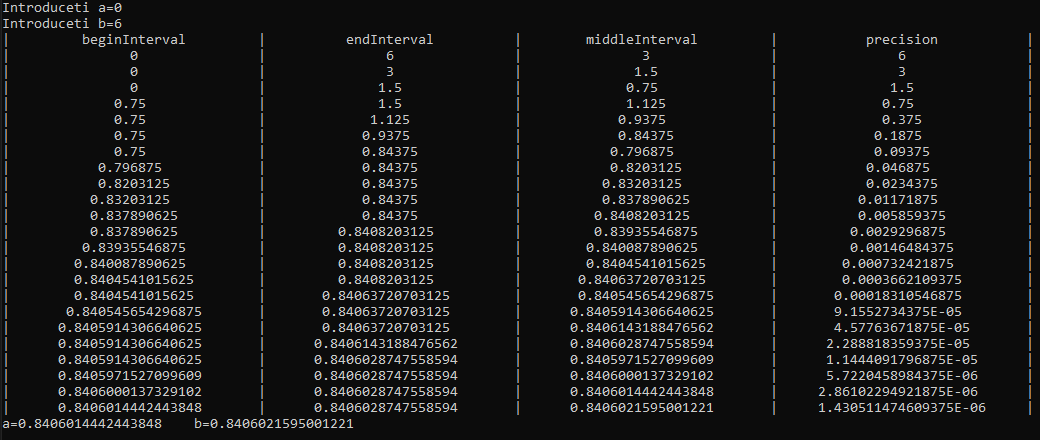
\includegraphics[width=0.8\textwidth]{assets/listings/bisection-output.png} \par

\clearpage
